%% This is file `elsarticle-template-1-num.tex',
%%
%% Copyright 2009 Elsevier Ltd
%%
%% This file is part of the 'Elsarticle Bundle'.
%% ---------------------------------------------
% \documentclass[preprint,12pt]{elsarticle}
%% Use the option review to obtain double line spacing
%% \documentclass[preprint,review,12pt]{elsarticle}

%% Use the options 1p,twocolumn; 3p; 3p,twocolumn; 5p; or 5p,twocolumn
%% for a journal layout:
% \documentclass[final,1p,times]{elsarticle}
% \documentclass[final,1p,times,twocolumn]{elsarticle}
%% \documentclass[final,3p,times]{elsarticle}
%% \documentclass[final,3p,times,twocolumn]{elsarticle}
%% \documentclass[final,5p,times]{elsarticle}
\documentclass[final,5p,times,twocolumn]{elsarticle}

%% The graphicx package provides the includegraphics command.
% \usepackage{graphicx}
%% The amssymb package provides various useful mathematical symbols
% \usepackage{amssymb}
%% The amsthm package provides extended theorem environments
%% \usepackage{amsthm}

%% The lineno packages adds line numbers. Start line numbering with
%% \begin{linenumbers}, end it with \end{linenumbers}. Or switch it on
%% for the whole article with \linenumbers after \end{frontmatter}.
% \usepackage{lineno}

%% \biboptions{comma,round}

% \biboptions{}
\usepackage{nameref}
\usepackage{siunitx}


% include graphics
\usepackage{graphicx}
\graphicspath{ {figures/} }

% include pdfs
\usepackage{pdfpages}


%% using bibtex with biber
\usepackage[
    backend=biber,
    style=nature,
    sortlocale=de_DE,
    url=false,
    doi=true,
    eprint=false
]{biblatex}
\addbibresource{reference.bib}


\journal{Modern Pathology}
\begin{document}


\begin{frontmatter}

%% Title
\title{Investigating semi-automated ki67 scoring efficacy}
%% Authors
\author[music]{Tian Yu Liu}
\author[molgen]{Peiqi Wang}
\author[cf]{Susan J. Done\corref{cor}}
\ead{Susan.Done@uhn.ca}
%% address
\cortext[cor]{Principal corresponding author}
\address[music]{Faculty of Music, Univeristy of Toronto, ON, Canada}
\address[molgen]{Department of Molecular Genetics and Microbiology, University of Toronto, Canada}
\address[cf]{The Campbell Family Institute for Breast Cancer Research, Canada}

\begin{abstract}
300words, work done, result obtained, conclusions drawn. filled in later


% \begin{itemize}
% \item Bullet point one
% \item Bullet point two
% \end{itemize}
%
% \begin{enumerate}
% \item Numbered list item one
% \item Numbered list item two
% \end{enumerate}

% \begin{table}[h]
% \centering
% \begin{tabular}{l l l}
% \hline
% \textbf{Treatments} & \textbf{Response 1} & \textbf{Response 2}\\
% \hline
% Treatment 1 & 0.0003262 & 0.562 \\
% Treatment 2 & 0.0015681 & 0.910 \\
% Treatment 3 & 0.0009271 & 0.296 \\
% \hline
% \end{tabular}
% \caption{Table caption}
% \end{table}


\end{abstract}

\begin{keyword}
ki67 \sep breast cancer
\end{keyword}

\end{frontmatter}

%%
%% Start line numbering here if you want
%%
\linenumbers

%% main text
\section*{Introduction}

Ki-67 is a human nuclear protein detected exclusively in the active phases of the cell cycle, namely $G_1$, $S$, $G_2$, and mitosis, while absent in the resting $G_0$ phase.\cite{Gerdes1984} It is expressed in virtually cells of every tissue origin and is highly sensitive to cell cycle changes, making it an ideal marker for quantifying uncontroled proliferation, a hallmark of cancer. Unsurprisingly, Ki-67 immunohistochemical (IHC) staining of human neoplasmic cell has emerged as a rapid and cost-effective analytics capable of determining the growth fraction of tumour cell populations,  \cite{Scholzen2000} The use of Ki-67 labelling index, or the percentage of Ki-67-positive cells, has great prognostic potential particuarly in carcinomas of the breast, where a multitude of studies reported the use of Ki-67 labeling index in predicting disease free/overall survival and tumour recurrence \cite{Stuart-Harris2005, DeAzambuja2007} as well as in guiding neoadjuvant chemotherapy. \cite{Jones2009, Nishimura2010, Fasching2011} Practically, Ki-67 labeling index served as a feasible alternative to gene signature based assessments such as OncotypeDx in cancer subtyping when used in conjunction with established breast histopathological markers such as ER, PgR, and HER2. \cite{Cuzick2011} Despite its apparent value in cancer prognosis, widespread use of Ki-67 labeling index in clinical pathology is hampered by the lack of standardization and suffers from substantial intra- amd interobserver variability. \cite{Dowsett2011a, Polley2013a} Although recommendations and guidlines exist in an effort to harmonize such variability, \cite{Polley2015} the choice of scoring methods and selection of cutoff for Ki-67 positivity remain a subject of debate. One promising approach to the problem utilizes digital image analysis (DIA), which reduces interobserver variability and alleviatas labor intensive work. In some cases, DIA was reported to outperform traditional manual scoring methods. \cite{Stalhammar2016}

In this study, we evaluated the efficacy and reproducibility of two digital image analysis methods - Aperio ePathology and Definiens Tissue Studio. Additionally, we measured their agreement to a set of manual scores previously identified to be a predictor of ipsilateral breast relapse in the the Toronto-British Columbia (TBC) trial patient cohort. \cite{Liu2015}

\cite{Scholzen2000}

\section*{Materials and Methods}

\subsection*{Patients and Sample Collection}
A subset of patient cohort from the TBC trial were used for this study. The TBC trial consists of node-negative patients who were older than 50 years of age randomly assigned to receive tamoxifen alone or tamoxifen and breast radiotherapy after breast-conserving surgery. \cite{Fyles2009} Tissue microarrays were constructed using a triplicate of \SI{0.6}{\milli\metre} tumour cores from formalin-fixed, paraffin-embedded blocks. A total of 6 TMA blocks, amounting to 278 cases, where used for subsequent IHC and image analysis.

\subsection*{Ki-67 Immunohistochemistry}

TMA blocks were cut in \SI{0.5}{\micro\metre} sections and incubated with monoclonal MIB-1 antibody (Dako) at [time, temperature] and counter-stained with hematoxylin. [more on positive negative control and specifics of staining, are they all from the same staining]

\subsection*{Scoring Methodologies}

\subsubsection*{Manual Assessment}
A trained pathologist counted the number of brown staining for at least 100 cells within tumour hot spot, or areas in which Ki-67 staining is predominant, for each core. The total number of nucleus and positively stained nucleus over the span of three cores were summed and the Ki-67 labeling index was calculated for each case. 10\% of the samples were randomly chosen and rescored for quality assurance.

\subsubsection*{Digital Image Analysis (DIA)}
Stained sections were scanned by [detail regarding scaninng process]. To assess reproducibility of DIA, specifically the Aperio system, 2 pathologists independently marked tumour region of interest. Settings for the detection algorithm were adjusted for by another experienced pathologist and used in both set of annotations. Annotated images were analyzed to quantify inter-rater reliability when using a DIA method. To assess the agreement of DIA method to the manual scores, the same set of images were analyzed using the Definiens system in addition to the Aperio system. In this case, a technician marked tumour areas in a few cores, which trained the software to recognize tumour areas for every other cases.

\subsection*{Statistics}
Data distribution cross different scoring methods were visulized using boxplot, accompanied by summary statistics. Inter-rater reliability (IRR) was quantified using a two-way mixed, average-measures intraclass correlation coefficient(ICC) to assess the degree that raters provide absolute agrement in their ratings of Ki-67 labeling index using the Aperio system. An ICC close to 1 represents high reliability. Similarly, ICC was used to assess the degree that different scoring methods agree on the same patient cohort. Bland-Altman plot was used to visualize agreement between results from manual assessment and the two DIA methods. \cite{Bland1986} 95\% confidence interval for the limits of agreement as well as the mean of difference was calculated based on an alpha of 0.05. High agreement between scoring methods equates to a mean of differences centered about zero with a small standard deviation. Fleiss Kappa were calculated based a cutoff for Ki-67 labeling index of 15 to quantify the practicality of correctly classfying a core into clinically relevant groups , namely Ki-67 low and Ki-67 high.


\section*{Results}

\subsubsection*{Overall distribution}
Boxplot of untransformed Ki-67 labeling index as well as summary statistics of log2-transformed Ki-67 labeling index were presented in Figure ~\ref{boxplot}, and Table ~\ref{summaryStatistics}. The Aperio system tended to overestimate Ki-67 labeling index; whereas the Definiens system corresponded well to manual assessment.


\subsubsection*{Inter-rater Reliability Using a DIA Method}
ICC between two raters using the the Aperio system was 0.675 (95\%CI: 0.534-0.768) The resulting ICC could only be considered fair, suggesting that a considerable amount of error was introduced by annotating appropriate tumour areas for analysis. \cite{Cicchetti1994} Additionally, the Kappa statistics was fairly low when comparing how two raters agree using the Aperio system alone (0.256).


\subsubsection*{Agreement of DIA methods to Manual Assessment}

Bland-Altman plot for every DIA method with respect to corresponding manual assessment was listed in Figure ~\ref{baplot1}, ~\ref{baplot2}, ~\ref{baplot3}. The limits of agreement using the Aperio system against manual assessment were -53.4(95\%CI: -57.2--49.5) to 14.0 (95\%CI: 10.1-17.8) with a mean of difference of -19.7 (95\%CI: -21.9-17.8) and -51.8 (95\%CI: -56.2--12.6) to 21.5 (95\%CI: -17.7-25.9) with a mean of -15.1 (95\%CI: -47.3-17.0) respectively. It is apparent that the Aperio system systematically overestimated Ki-67 labeling index by a large margin, perhaps a direct result of inaccurate calibration procedure as there is no a priori settings for the algorithm. The limits of agreement using the Definiens system against manual assessment were -10.383 (95\%CI: -12.314--8.451) to  10.960 (95\%CI:  9.029-12.892) with a mean difference of 0.289 (95\%CI: -0.826-1.404).  High agreement was observed with minimal bias. This may be attributable to better detection algorithms and design of workflow, where raters would necessarily rely on computer algorithm to detect tumour region. ICC of two raters using the Aperio system when compared directly to the manual assessment was 0.185 (95\%CI -0.25-0.475) and 0.333 (95\%CI -0.166-0.595) respectively; whereas ICC of rater using the Definiens system when compared to the manual assessment was 0.935 (95\%CI 0.903-0.957). Such dichotomizing CCI implicated a substantial difference in the analytical accuracy of different DIA methods. Kappa statistics were -0.142 and 0.127 respectively for using the Aperio system, indicating the inability of the Aperio system to classify cores into clinically relevant groups. For the Definiens system, the Kappa statistics was 0.787, indicating high agreement in making clinically relevant classifications.


\section*{Discussions}
interpretation of significance of findings, relate to other works, further research directions

\printbibliography


\newpage
%% figures and tables



\begin{figure}
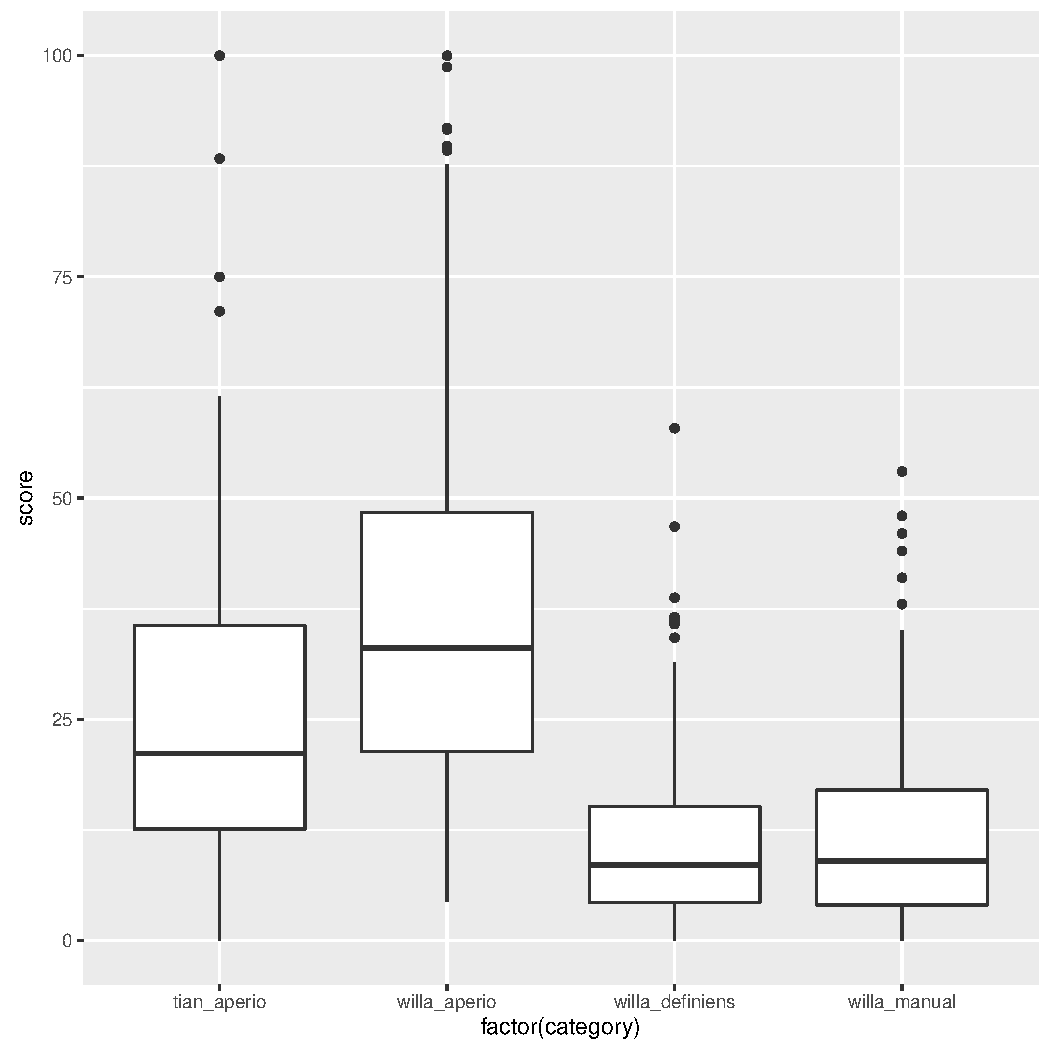
\includegraphics[width = 11cm]{boxplot}
\centering
\caption{{\bf Summary boxplot of Ki-67 labeling index}}
\label{boxplot}
\end{figure}




%latex.default(s)%
\begin{table}[!tbp]
\begin{center}
\begin{tabular}{lrrrr}
\hline\hline
\multicolumn{1}{l}{s}&\multicolumn{1}{c}{tian\_aperio}&\multicolumn{1}{c}{willa\_aperio}&\multicolumn{1}{c}{willa\_definiens}&\multicolumn{1}{c}{willa\_manual}\tabularnewline
\hline
Min.&$-3.32$&$2.15$&$-3.32$&$-3.32$\tabularnewline
1st Qu.&$ 3.67$&$4.42$&$ 2.14$&$ 2.04$\tabularnewline
Median&$ 4.41$&$5.05$&$ 3.11$&$ 3.19$\tabularnewline
Mean&$ 4.35$&$4.95$&$ 2.94$&$ 2.79$\tabularnewline
3rd Qu.&$ 5.16$&$5.60$&$ 3.93$&$ 4.10$\tabularnewline
Max.&$ 6.65$&$6.65$&$ 5.86$&$ 5.73$\tabularnewline
\hline
\end{tabular}\end{center}
\caption{{\bf Summary statistics for log2-transformed Ki-67 labeling index}}
\label{summaryStatistics}

\end{table}

\begin{figure}
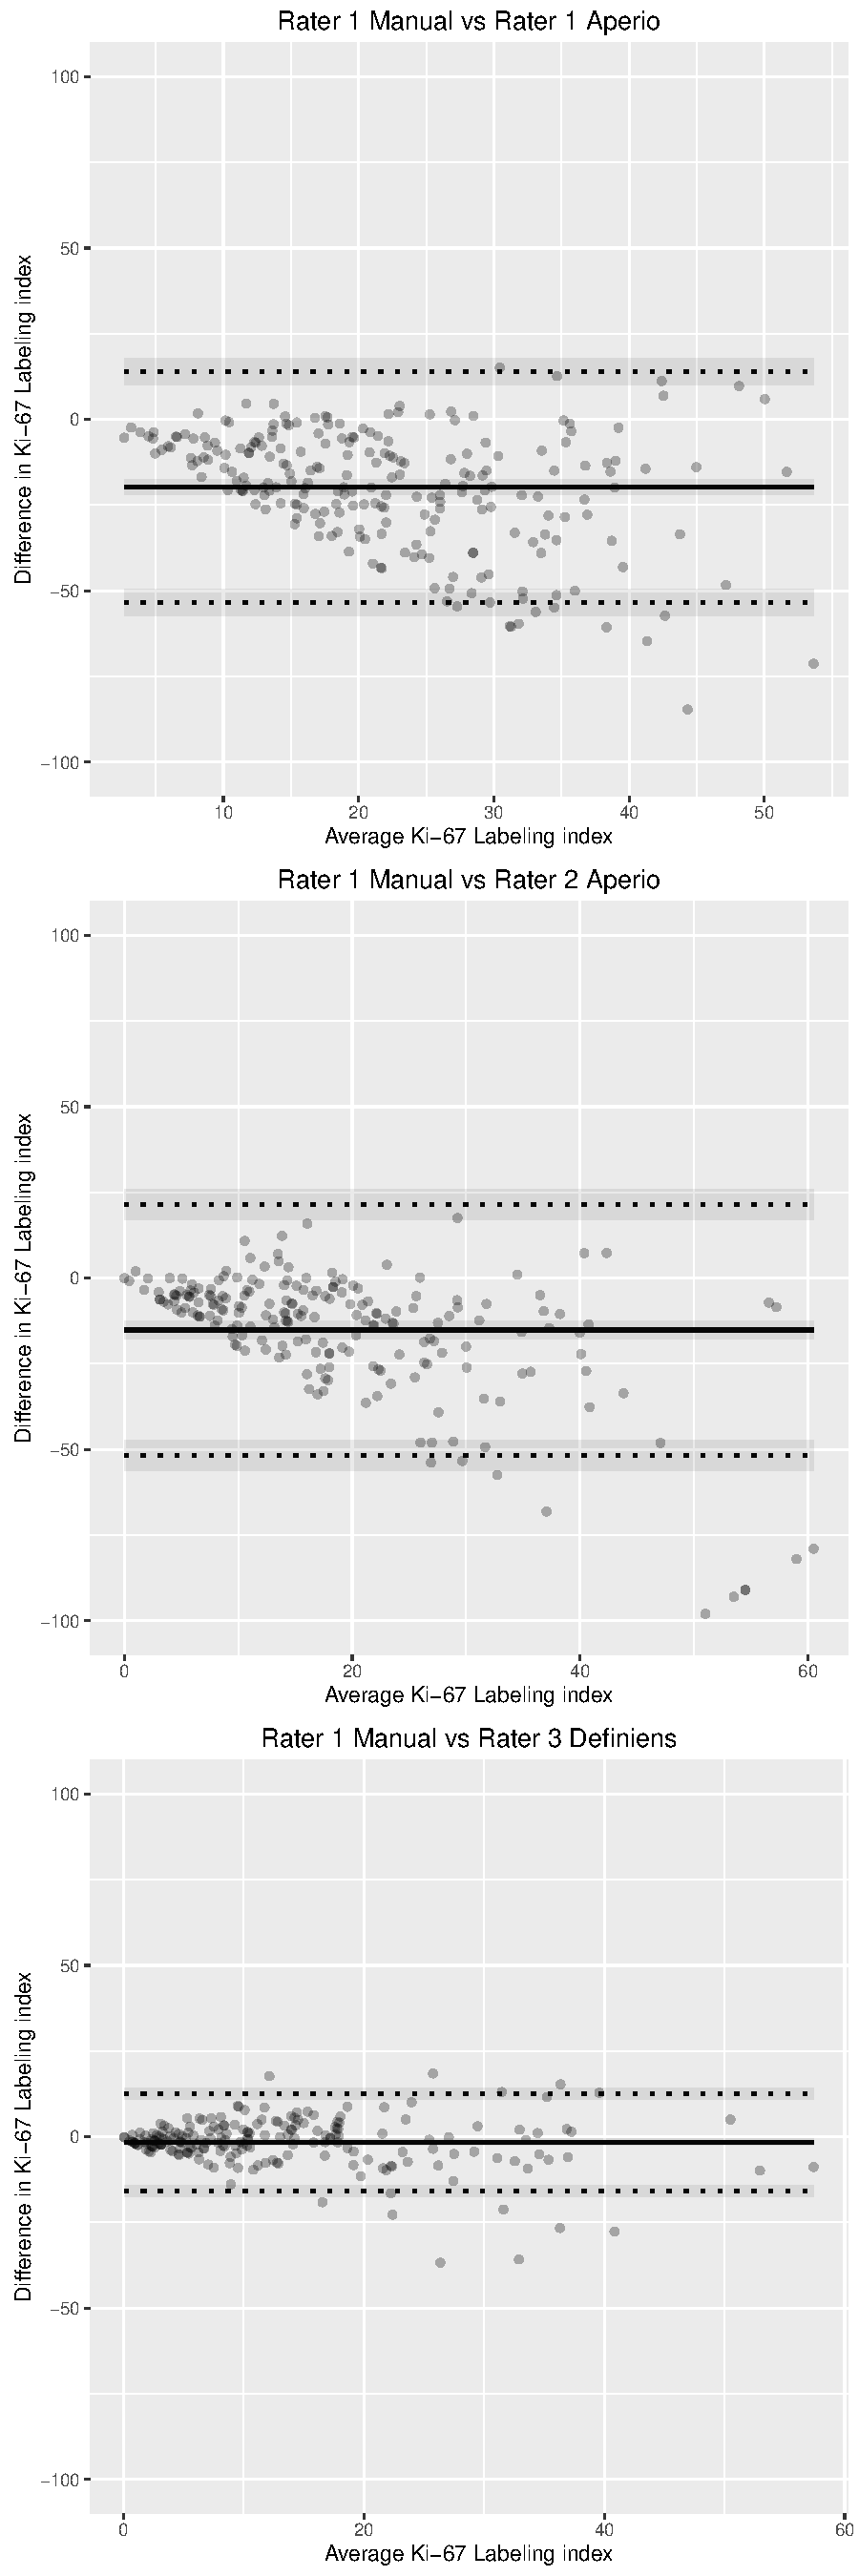
\includegraphics[page=1, scale=0.4]{baplot.pdf}
\centering
\caption{{\bf Bland-Altman Plot for Aperio DIA rater 1 vs. manual assessment}}
\label{baplot1}
\end{figure}


\begin{figure}
\includegraphics[page=2, scale=0.4]{baplot.pdf}
\centering
\caption{{\bf Bland-Altman Plot for Aperio DIA rater 2 vs. manual assessment}}
\label{baplot2}
\end{figure}


\begin{figure}
\includegraphics[page=3, scale=0.4]{baplot.pdf}
\centering
\caption{{\bf Bland-Altman Plot for Definiens DIA vs. manual assessment}}
\label{baplot3}
\end{figure}













\end{document}

%%
%% End of file `elsarticle-template-1-num.tex'.
